% ~ 12 pages
\chapter{Identification of Hadronic Tau Lepton Decays using Neural Networks}
\label{sec:rnn}

This chapter investigates the application of neural networks for tau
identification. First it will be shown that a multi-layer perceptron (MLP) can
achieve a classification performance comparable to the optimised BDT from the
previous chapter. Subsequently, novel sequence learning techniques are employed
to create classifiers operating on sequences of reconstructed objects. For this
the recurrent neural networks based on the LSTM architecture are used to create
classifiers operating on tracks in the inner detector and clusters in the
calorimeter. In this context a tau identification algorithm using purely
calorimetric information is developed and its potential application for reducing
the trigger-rate of a di-tau trigger at the \emph{High Luminosity LHC} (HL-LHC)
is presented. Finally, a model combining the multi-layer perceptron and the
recurrent networks operating on track- and cluster-information is developed.

\section{Identification using Feedforward Neural Networks}
\label{sec:ffnn_id}

Before proceeding to sequence classification techniques the viability of neural
networks to perform tau identification using simple network architectures is
shown. This will aid as a introduction to important concepts when training
neural networks. Moreover, the resulting network will be used as a building
block in the final model.

The optimised BDT from Chapter~\ref{sec:bdt} will be used as a reference for the
investigations in this chapter. Therefore the models will be trained and
evaluated using the same event samples, preselection and reweighting scheme
presented in Section~\ref{sec:bdt_eventsim}. In contrast to hold-out validation
used in the previous chapter, the full event sample is now randomly split into a
training, validation and testing sample. The samples have a relative size of
\SI{40}{\percent}, \SI{10}{\percent} and \SI{50}{\percent}, respectively. The
purpose of the training and testing sample is the same as before, however the
validation sample is monitored during the training process and used to perform
model selection and early stopping. A separate sample, as opposed to the testing
sample, is used to avoid introducing biases in the performance measurement on
the testing sample. This approach will be used for the remainder of this
chapter.

To reproduce the performance of the BDT-based tau identification a multi-layer
perceptron (MLP) with two hidden layers~(cf.\ Section~\ref{sec:nn_feedforward})
is used. The MLP uses the same input variables used for the optimised BDT.
Moreover, the input variables are standardised by subtracting the mean and
dividing by the standard deviation derived from the distributions in the
training sample. This preprocessing step is important as the gradient descent
algorithm used for training is sensitive to variables on different scales. The
input layer of the MLP consists of 9 (10) neurons corresponding to the input
variables for the 1-prong (3-prong) identification. Both hidden layers of the
MLP have a size of 128 units, which are activated by rectified linear units
(ReLU). A single output neuron using the logistic sigmoid as its activation
function, therefore returning probabilities of an event being signal-like. The
binary cross-entropy loss function is used and minimised by the \emph{Adam}
optimiser.

\begin{figure}[htb]
  \begin{subfigure}[t]{0.48\textwidth}
    \centering
    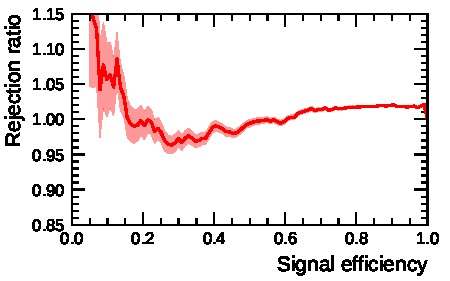
\includegraphics{./figures/rnn/mlp/mlp_bdt_ratio_1p.pdf}
    \subcaption{1-prong}
  \end{subfigure}\hfill
  \begin{subfigure}[t]{0.48\textwidth}
    \centering
    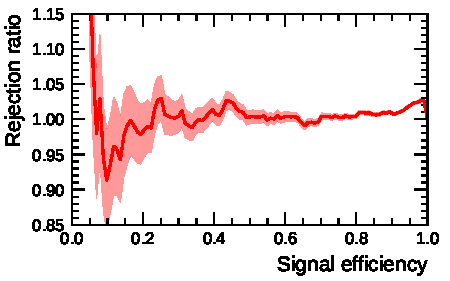
\includegraphics{./figures/rnn/mlp/mlp_bdt_ratio_3p.pdf}
    \subcaption{3-prong}
  \end{subfigure}
  \caption{Ratio of background rejection of the MLP and the optimised BDT as a
    function of signal efficiency. The band indicates the $1\sigma$-interval.}
  \label{fig:roc_mlp_bdt_comparison}
\end{figure}

In Figure~\ref{fig:roc_mlp_bdt_comparison} the ratio of rejection of the MLP and
the optimised BDT is depicted as a function of the signal efficiency. The
1-prong MLP shows comparable performance above \SI{60}{\percent} signal
efficiency, which approximately corresponds to the tight working point. Over the
intermediate efficiency range the performance degrades slightly. The 3-prong MLP
is consistent with the performance of the optimised BDT identification with a
small improvement at high efficiencies.

To summarise, both the 1- and 3-prong MLP achieve similar performance
characteristics as the optimised BDT from Chapter~\ref{sec:bdt}. The results
show that neural networks are a viable method to perform tau identification.

\section{Identification using Recurrent Neural Networks}
\label{sec:rnn_id}

Thus far approaches of tau identification use high-level variables that
summarise properties of reconstructed objects in the detector. This has the
advantage that identification can be understood and investigations into
systematic errors are simplified. However, discriminative power can be lost when
transitioning from low- to high-level variables. Therefore, an approach is
presented capturing low-level information by employing sequence classification
techniques. A general description of the method is given and subsequently
applied to reconstructed tracks and clusters in the calorimeter.

\subsection{General Description}
\label{sec:rnn_descr}

\begin{figure}[ht]
  \centering
  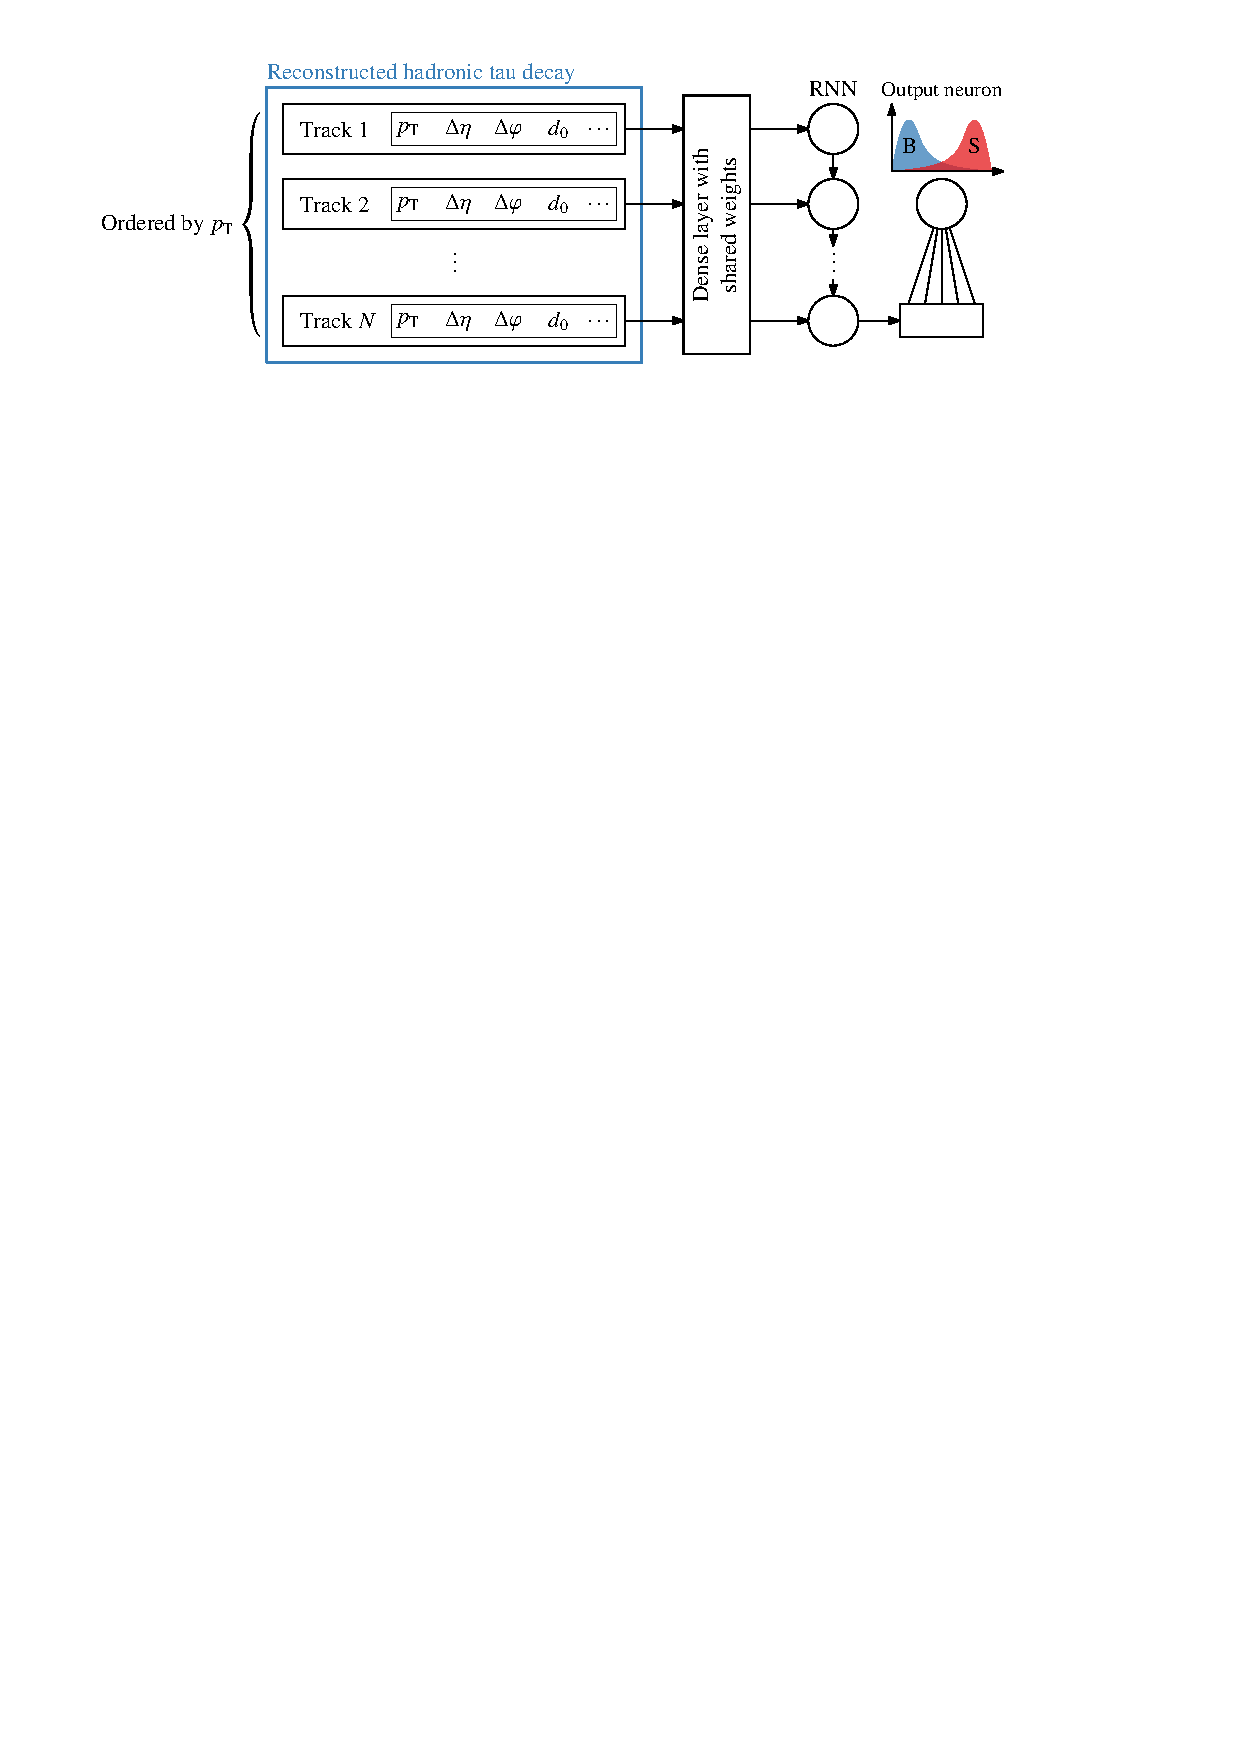
\includegraphics[scale=0.9]{./figures/rnn/track_rnn_schematic.pdf}
  \caption{Schematic of the Track-RNN}
  \label{fig:track_rnn_schematic}
\end{figure}


- Motivation:

+ Track-based variables contribute with a large majority of rejection -- further
exploit track information

+ Current tuning of the track classification: found to be suboptimal isolation
category for tau identification switched to modified isolation tracks (only
trained to classifiy tau decays not for tracks of dijet events)

+ Information might be lost when only considering a small selection of
high-level variables (e.g. no information on momentum of individual tracks or
their distance to the tau axis, only summarising quantities like momentum
fractions, mean distances etc.) (the same is true for cluster information)

- Take sequences of reconstructed objects. In this case tracks and clusters and
their properties. Also properties of the global tau.

- Pass them one by one to a recurrent neural network (ordering)

- Perform tau identification. Classifying a sequence of objects

- Describe base architecture. Input -- Masking -- Shared dense -- LSTM -- Dense (sigmoid)

- Explain what shared dense does

- Hyperparams mainly optimised for 1-prong operation

Hyperparameters do not claim to be optimal. Roughly optimised by hand observing the validation loss during training.


\todo[inline]{Correlation with output / label}
\todo[inline]{Group-wise variable importances for RNN}


A shared
dense layer applies an affine transformation to the input variables of each PFO.
Afterwards the transformed sequences are fed into the recurrent layer returning
a single vector of activations.
The activations of both branches are
concatenated \todo{shorten this as it will be explained in the RNN-ID part} and
passed through a network containing three dense layers.



\subsection{Track-RNN}
\label{sec:rnn_tracks}

\todo[inline]{ROC-Curves}

\todo[inline]{Check whether the missing tau hits in the ID are a problem at
  high-pt.}

Using reconstructed tracks with a minimum transverse momentum of
\SI{400}{\mega\electronvolt} (already applied in track reconstruction).

Input Variables: Transverse momentum of the track $p_\text{T}^\text{track}$
measured in the tracking system; Absolute value of the transverse impact
parameter $d_0$ with respect to the associated vertex; Distance of closest
approach to the primary vertex in the $z$-$r$ plane $z_0 \sin\theta$ where
$\theta$ is the polar angle of the track \todo{Axis is corrected, use
  $\sin\theta$ instead of $z_0$ due to expected larger error in forward
  direction}; Signed angular distance of track and tau axis $\Delta \eta$ and
$\Delta \varphi$; Electron probability from high-threshold hit information in
the TRT $p_\text{HT}$; Number of hits in IBL $N_\text{hit}^\text{IBL}$, the
three pixel layers (B-layer, 1 and 2) $N_\text{hit}^\text{pixel}$ and the SCT
$N_\text{hit}^\text{SCT}$ (dead sensors crossed by the reconstructed track are
also counted as hits).

Variable importances:
\begin{enumerate}
\item $d_0$ and $z_0 \sin\theta$
\item $p_\text{T}^\text{track}$ and $p_\text{T}^\text{jet}$
\item $\Delta \eta$ and $\Delta \varphi$
\item \texttt{nInnermostPixelHits}, \texttt{nPixelHits} and \texttt{nSCTHits}
\item \texttt{eProbabilityHT}
\end{enumerate}

\begin{table}[ht]
  \centering
  {\small\begin{tabular}{p{5cm}S[table-format=1.4(4)]S[retain-explicit-plus, table-format=+2.1]}
  \toprule
  {Variables} & {Validation loss} & {Loss increase} \\
  \midrule
  \parbox[c]{\hsize}{Impact parameter \newline $d_0$, $z_0 \sin\theta$}
          & 0.2831 +- 0.0005 & + 48.4 \,\si{\percent} \\[1.2em]
  \parbox[c]{\hsize}{Transverse momentum \newline $p_\text{T}^\text{track}$, $p_\text{T}^\text{jet}$}
          & 0.2410 +- 0.0007 & + 26.3 \,\si{\percent} \\[1.2em]
  \parbox[c]{\hsize}{Angular distance \newline $\Delta \eta$, $\Delta \varphi$}
          & 0.2304 +- 0.0003 & + 20.8 \,\si{\percent} \\[1.2em]
  \parbox[c]{\hsize}{Hits in ID \newline $N_\text{hit}^\text{pixel}$, $N_\text{hit}^\text{SCT}$}
          & 0.2036 +- 0.0013 & + 6.7 \,\si{\percent} \\[1.2em]
  \parbox[c]{\hsize}{Electron probability (TRT) \newline $p_\text{HT}$}
          & 0.1930 +- 0.0004 & + 1.2 \,\si{\percent}\\
  \bottomrule
\end{tabular}

%%% Local Variables:
%%% mode: latex
%%% TeX-master: "../mythesis"
%%% End:
}
  \caption{Variable importance table}
\end{table}

\todo{use 10 tracks}

\todo[inline]{uses 32 lstm units}

\todo{Variable importance (in groups?)}

\todo{\SI{40}{\percent} training, \SI{10}{\percent} validation and \SI{50}{\percent} testing}

What has been tested:
\begin{itemize}
\item Ordering $p_\text{T}$
\item Preprocessing
\item Variables: Track classification
\item
\end{itemize}

\begin{figure}[ht]
  \begin{subfigure}[t]{0.48\textwidth}
    \centering
    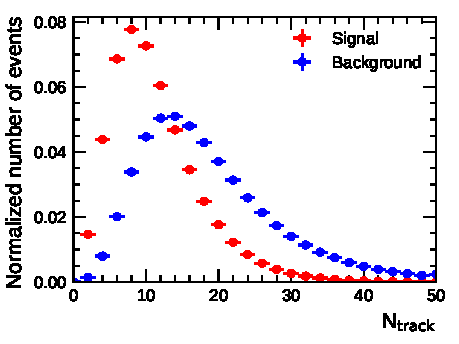
\includegraphics{./figures/rnn/ntrk_1p.pdf}
    \subcaption{NTracks for 1-prong taus. The reco.\ three prong distribution is
      similar with the difference being that at least three tracks are
      required.}
  \end{subfigure}\hfill
  \begin{subfigure}[t]{0.48\textwidth}
    \centering
    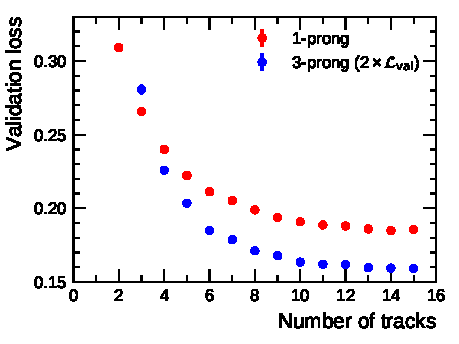
\includegraphics{./figures/rnn/nscan/track_1p_3p.pdf}
    \subcaption{Val.\ loss vs.\ nTracks. Errors are of the
      order of the marker size.}
  \end{subfigure}
  \caption{Tracks associated with a tau}
  \label{fig:rnn_ntracks}
\end{figure}

\begin{itemize}
\item Motivation (i.e. \texttt{SumPtTrkFrac} \& MVA-tracking)
\item Architecture (mention rough optimisation by hand while monitoring
  validation loss)
\item Preprocessing
\item Input variables \& correlation with true (or predicted?) class labels.
  Partial dependence plots? Variable importance?
\item Standalone performance vs. BDT-based ID
\end{itemize}

\begin{itemize}
\item Validation loss vs.\ sample size
\end{itemize}

\begin{figure}[ht]
  \begin{subfigure}[t]{0.48\textwidth}
    \centering
    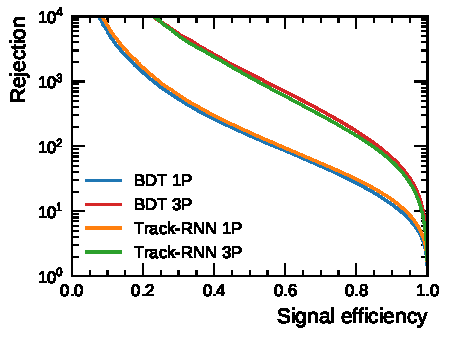
\includegraphics{./figures/rnn/track/roc.pdf}
    \subcaption{ROC-curves for 1-prong (1P) and 3-prong (3P) tau
      identification.}
  \end{subfigure}\hfill
  \begin{subfigure}[t]{0.48\textwidth}
    \centering
    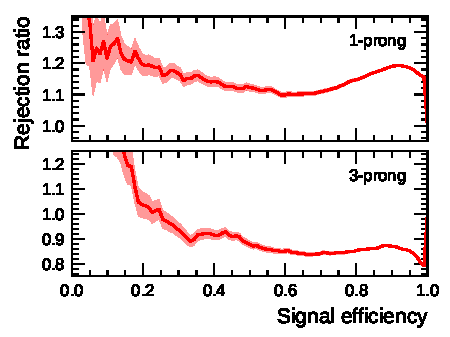
\includegraphics{./figures/rnn/track/ratios.pdf}
    \subcaption{Rejection ratio of the Track-RNN with respect to the optimised
      BDT.}
  \end{subfigure}
  \caption{Classification performance of the Track-RNN compared to the optimised
    BDT for tau identification.}
  \label{fig:track_rnn_roc_ratios}
\end{figure}

\begin{figure}[ht]
  \centering
  \begin{subfigure}[t]{0.48\textwidth}
    \centering
    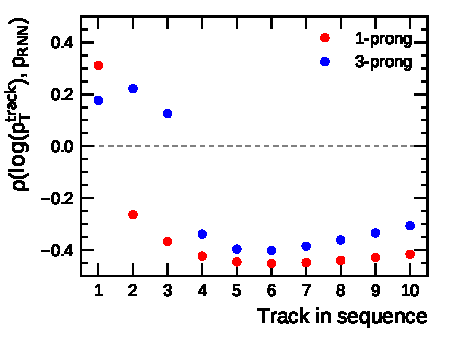
\includegraphics{./figures/rnn/track/pt_corr.pdf}
    \subcaption{}
  \end{subfigure}\hfill
  \begin{subfigure}[t]{0.48\textwidth}
    \centering
    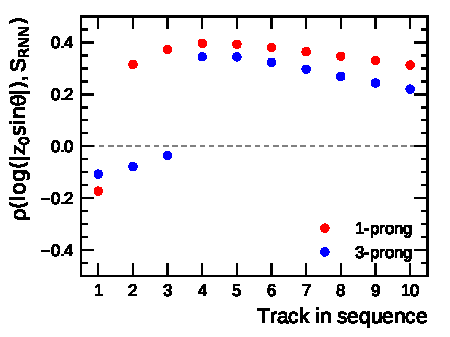
\includegraphics{./figures/rnn/track/z0_corr.pdf}
    \subcaption{}
  \end{subfigure}
  \caption{Classification performance of the Track-RNN compared to the optimised
    BDT for tau identification.}
  \label{fig:track_rnn_roc_ratios}
  \todo[inline]{Explain that $\Delta R$ is similar to $z_0$ i.e.\ close to axis
    for leading 1 or 3 tracks far for rest. Ref to plot in appendix.}
\end{figure}


\subsection{Cluster-RNN}
\label{sec:rnn_clusters}

\todo[inline]{ROC-Curves}

\todo{Idea is to use cluster moments as a proxy for cell-based variables}

Variable evolution:
\begin{itemize}
\item Energy fractions in PS, EM1, EM2, EM3 (only small improvement)
\item $\Delta R \rightarrow \Delta \phi, \Delta \eta$
\item Importance: 1.\ Direction of the cluster $\Delta \phi, \Delta \eta$; 2.\
  Energy and pt of the jet; 3.\ Cluster moments; 4.\ Energy fractions
\end{itemize}

\begin{figure}[ht]
  \begin{subfigure}[t]{0.48\textwidth}
    \centering
    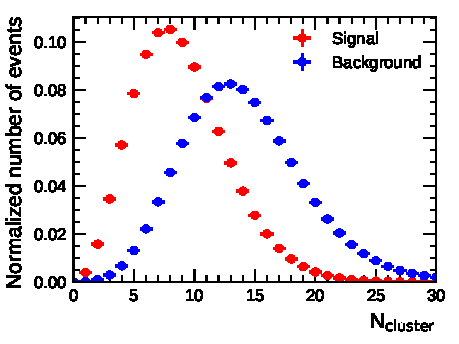
\includegraphics{./figures/rnn/ncls_1p.pdf}
    \subcaption{NCluster for 1-prong taus}
  \end{subfigure}%
  \begin{subfigure}[t]{0.48\textwidth}
    \centering
    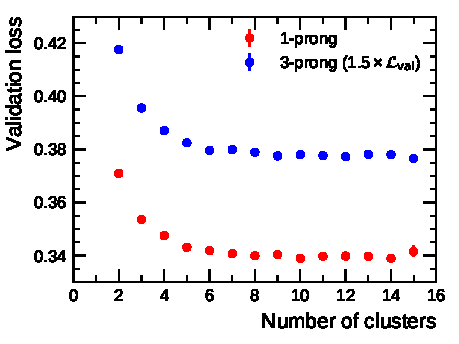
\includegraphics{./figures/rnn/nscan/cluster_1p_3p.pdf}
    \subcaption{Val.\ loss vs.\ nCluster}
  \end{subfigure}
  \caption{Clusters associated with a tau}
  \label{fig:rnn_nclusters}
\end{figure}

\todo{Use 6 clusters}

\begin{itemize}
\item Input variables \& correlation with true class labels. Partial
  dependence plots?
\item Validation loss vs. number of clusters
\item Standalone performance
\end{itemize}


\begin{figure}[ht]
  \begin{subfigure}[t]{0.48\textwidth}
    \centering
    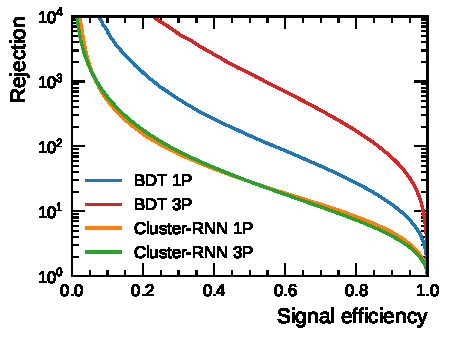
\includegraphics{./figures/rnn/cluster/roc.pdf}
    \subcaption{ROC-curves for 1-prong (1P) and 3-prong (3P) tau
      identification.}
  \end{subfigure}\hfill
  \begin{subfigure}[t]{0.48\textwidth}
    \centering
    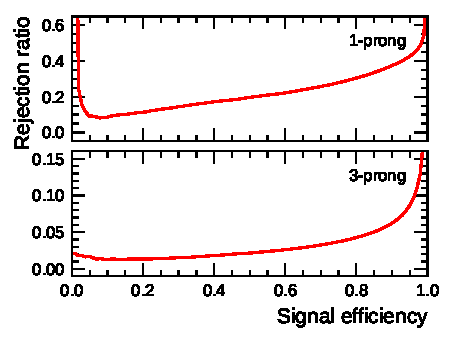
\includegraphics{./figures/rnn/cluster/ratios.pdf}
    \subcaption{Rejection ratio of the Cluster-RNN with respect to the optimised
      BDT.}
  \end{subfigure}
  \caption{Classification performance of the Cluster-RNN compared to the optimised
    BDT for tau identification.}
  \label{fig:cluster_rnn_roc_ratios}
\end{figure}

\subsubsection{Di-Tau Identification at the High Luminosity LHC}
\label{sec:hlt_rate_reduction}

The Phase-II upgrade of the LHC called the High Luminosity LHC (HL-LHC) is
foreseen to be finished by 2026. It will increase the instantaneous luminosity
to~\num{5}\,--\,\SI{7.5e34}{\per\square\centi\metre\per\second} at a
centre-of-mass energy
of~$\sqrt{s} = \SI{14}{\TeV}$~\cite{hl_lhc_prelim_design_report}. This
corresponds to a five- to sevenfold increase in luminosity with respect to the
beginning of Run-II and increases the average number of interactions per bunch
crossing to up to \num{200}. The increase in particle density poses a challenge
to the trigger systems and reconstruction algorithms.

An upgrade of the ATLAS trigger with a \emph{Global Trigger System} aims to
provide access to the full calorimeter granularity with topoclustering and jet
finding using iterative jet algorithms in regions of
interest~\cite{phase_2_scoping}. This aims to improve the identification of
physics objects at trigger-level to cope with increasing trigger rates due to
pile-up. Due to the availability of full calorimeter granularity, offline
reconstructed taus can be used to give prospects of the potential performance of
a di-tau trigger in the HL-LHC environment.

A prospective study on the usage of the cluster-based RNN for identification of
taus in a di-tau trigger is given. Offline reconstructed taus are used as an
approximation to the objects at the Phase-II trigger. The study uses simulated
samples of~$\text{Z} / \text{DY} \to \tau \tau$ and dijets at HL-LHC conditions
with centre-of-mass energy~$\sqrt{s}=\SI{14}{\TeV}$ and average interactions per
bunch crossing~$\mu = 200$ (cf.\ Appendix~\ref{app:upgrade_samples}).

The cluster-based RNN identification is retrained on individual tau candidates
in the HL-LHC upgrade samples using the same preselection used for the BDT
identification in Chapter~\ref{sec:bdt} with the exception of any
tracking-related requirements. The leading and subleading tau with respect to
the reconstructed transverse momentum (using Run-II calibrations) are selected
in a given event, while additionally requiring truth-matched hadronic tau decays
for the signal sample. The RNN identification is applied to each tau
individually resulting in two identification scores per event. The leading and
subleading tau~$p_\text{T}$ and identification scores are combined in a logistic
regression to assign a single di-tau identification score to each event.

The accept-rate of \SI{200}{\kilo\hertz} of the higher-level triggers limits the
maximum trigger-rate of the di-tau trigger. Achieving this rate requires
$p_\text{T}$-thresholds on leading and subleading taus as well as application of
the di-tau identification. The thresholds should be kept low to ensure high
signal acceptance for physics analyses. For the purposes of this study a single
cut on the identification score is used to identify di-tau events.

\begin{figure}[htb]
  \centering
  \begin{subfigure}[t]{0.48\textwidth}
    \centering
    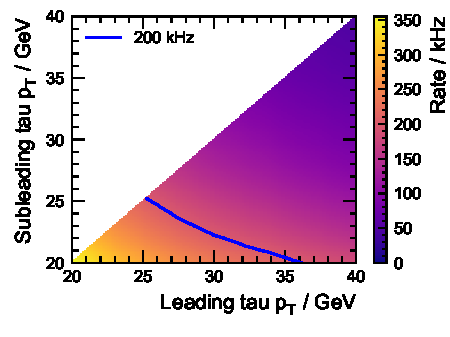
\includegraphics{./figures/rnn/trigger/pt_rate_reg.pdf}
    \subcaption{Trigger-rate after RNN-based identification as a function of
      leading and subleading tau offline $p_\text{T}$-threshold.}
    \label{fig:rate_vs_thresholds}
  \end{subfigure}\hfill
  \begin{subfigure}[t]{0.48\textwidth}
    \centering
    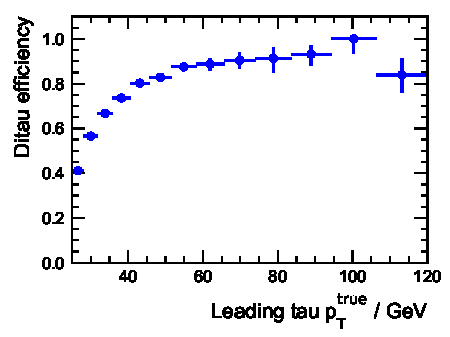
\includegraphics{./figures/rnn/trigger/taueff_reg.pdf}
    \subcaption{Di-tau selection efficiency of RNN-based identification with
      \SI{25}{\GeV} $p_\text{T}$-thresholds with respect to offline
      reconstructed tau lepton pairs measured in $\text{Z} \to \tau\tau$.}
    \label{fig:ditau_trigger_eff}
  \end{subfigure}
  \caption{Feasibility of using TopoClusters for a di-tau trigger at the
    HL-LHC.}
  \label{fig:rnn_ditau_trigger}
\end{figure}

The large dijet production cross section allows the assumption, that all
background events in the simulated sample correspond to a rate equal to the
average bunch crossing rate of~\SI{31.6}{\mega\hertz}. In
Figure~\ref{fig:rate_vs_thresholds} the trigger-rate is shown as a function of
the leading and subleading $p_\text{T}$-thresholds after applying di-tau
identification. The target rate can be achieved with a offline
$p_\text{T}$-threshold of \SI{25}{\GeV} on both taus.
Figure~\ref{fig:ditau_trigger_eff} shows the efficiency of the identification
using the leading and subleading \SI{25}{\GeV} threshold with respect to all
offline reconstructed di-tau pairs. The di-tau efficiency starts to plateau at
true visible transverse momentum~$p_\text{T}^\text{true} > \SI{40}{\GeV}$ of the
leading tau with an efficiency of approximately~\SI{90}{\percent}.

Ref.~\cite{phase_2_scoping} outlines a di-tau trigger with offline
$p_\text{T}$-threshold on the leading and subleading tau of \SI{40}{\GeV} and
\SI{30}{\GeV}, respectively. The approach using the cluster-based RNN
identification achieves the target rate at a reduced $p_\text{T}$-threshold
of~\SI{25}{\GeV}. The efficiency of the selection shows opportunities for
further enhancements by employing a proper tau energy calibration for HL-LHC
conditions and using a more advanced decision threshold for the di-tau
identification. The decision threshold could be loosened with increasing
transverse momentum to ensure a quicker turn-on and full efficiency at
high-$p_\text{t}$.

\subsection{Combined-RNN}
\label{sec:rnn_combined}

\todo[inline]{ROC-Curves}

\todo[inline]{Money plot: Rejection vs pt for Combined, Optimised BDT and
  Reference}

\begin{itemize}
\item Architecture
\item Performance w.r.t. BDT-ID
\item ROC of Track+Cluster \& Track+Cluster+IDvars
\item 3-prong cannot achieve Tau-ID level: Secondary vertex determination and
  invariant mass difficult
\end{itemize}

\todo[inline]{Study pile-up dependency of RNN vs BDT-ID}

%%% Local Variables:
%%% mode: latex
%%% TeX-master: "mythesis"
%%% End:
